\printconcepts

\exercise{T/F: The Chain Rule describes how to evaluate the derivative of a composition of functions.
}{T
}

\exercise{T/F: The Generalized Power Rule states that $\ds \frac{d}{dx}\Big( g(x)^n\Big) = n\big(g(x)\big)^{n-1}$.
}{F
}

\exercise{T/F: $\ds \frac{d}{dx}\big(\ln (x^2)\big) = \frac{1}{x^2}$.
}{F
}

\exercise{T/F: $\ds \frac{d}{dx}\big(3^x\big) \approx 1.1\cdot3^x$.
}{T
}

\exercise{T/F: $\ds \frac{dx}{dy} = \frac{dx}{dt}\cdot \frac{dt}{dy}$
}{T
}

\exercise{T/F: Taking the derivative of $f(x) = x^2\sin(5x)$ requires the use of both the Product and Chain Rules.}{T}

\printproblems

\exerciseset{In Exercises}{, compute the derivative of the given function.}{

\exercise{$f(x) = (4x^3-x)^{10}$\label{exer:02_05_06}}{$\fp(x) = 10(4x^3-x)^9\cdot(12x^2-1) = (120x^2-10)(4x^3-x)^9$}

\exercise{$f(t) = (3t-2)^{5}$}{$\fp(t) = 15(3t-2)^4$}

\exercise{$g(\theta) = (\sin \theta+\cos \theta)^3$}{$g'(\theta) = 3(\sin \theta+\cos \theta)^2(\cos \theta-\sin\theta)$}

\exercise{$h(t) = e^{3t^2+t-1}$\label{exer:02_05_09}}{$h'(t) = (6t+1)e^{3t^2+t-1}$}

\exercise{$f(x) = \big(x+\frac{1}{x}\big)^4$}{$\fp(x) = 4\big(x+\frac1x\big)^3\big(1-\frac{1}{x^2}\big)$}

\exercise{$p(x) = \left(x^2 - \dfrac{1}{x^2}\right)^6$}{$p'(x) = 12\left(x^2 - \dfrac{1}{x^2}\right)^5 \left(x + \dfrac{1}{x^3}\right)$}

\exercise{$f(x) = \cos (3x)$}{$\fp(x) = -3\sin(3x)$}

\exercise{$g(x) = \tan (5x)$}{$g'(x) = 5\sec^2(5x)$}

\exercise{$h(t) = \sin^4(2t)$}{$h'(t) = 8\sin^3(2t)\cos(2t)$}

\exercise{$p(t) = \cos^3(t^2+3t+1)$}{$p'(t) = -3\cos^2(t^2+3t+1)\sin(t^2+3t+1)(2t+3)$}

\exercise{$g(x) = \tan^2 x - \tan (x^2)$}{$g'(x) = 2(\tan x \sec^2 x - x \sec^2 (x^2))$}

\exercise{$w(x) = \sec (e^{x^3})$}{$w'(x) = 3x^2 e^{x^3}(\sec e^{x^3})(\tan e^{x^3})$}

\exercise{$f(x) = \ln (\cos x)$}{$\fp(x) = -\tan x$}

\exercise{$f(x) = \ln (x^2)$}{$\fp(x) = 2/x$}

\exercise{$f(x) = 2\ln (x)$}{$\fp(x) = 2/x$}

%\exercise{$g(r) = 4^r$}{$g'(r) = \ln 4\cdot 4^r$}

%\exercise{$g(t) = 5^{\cos t}$}{$g'(t) = -\ln 5\cdot 5^{\cos t}\sin t$}

\exercise{$g(t) = 15^2$}{$g'(t) = 0$}

\exercise{$r(x) = \dfrac{\sqrt {4x-3}}{x^2}$}{$r'(x) = \dfrac{-6(x-1)}{x^3 \sqrt {4x-3}}$}

\exercise{$f(x) = \dfrac {(3x^2 - 5)^4}{(2x^3-1)^2}$}{$\fp(x) = \dfrac {12x(2x^3-1)(3x^2 - 5)^3(x^2+5x-2)}{(2x^3-1)^4}$}

\exercise{$h(x)=[(2x+1)^{10} + 1]^{10}$}{$h'(x)=200(2x+1)^9[(2x+1){10}+1]^9$}

\exercise{$f(t)=\left[\left(1+ \dfrac{1}{t}\right)^{-1} + 1\right]^{-1}$}{$\fp(t)=\dfrac{-t^4}{(2t+1)(t+1)}$}

\exercise{$F(x)=2x(2x+1)^2 (2x+3)^3$}{$\Fp(x)=2(2x+1)(2x+3)^2(24x^2+26x+3)$}

%\exercise{$\ds m(w) = \frac{3^w}{2^w}$}{$m'(w) = \ln (3/2) (3/2)^w$}

%\exercise{$\ds h(t) = \frac{2^t+3}{3^t+2}$}{$\fp(x) = \frac{(3^t+2)\big((\ln 2) 2^t\big)-(2^t+3)\big((\ln 3)3^t\big)}{(3^t+2)^2}$}

%\exercise{$\ds m(w) = \frac{3^w+1}{2^w}$}{$m'(w) = \frac{2^w\big(\ln 3\cdot 3^w-\ln 2\cdot (3^w+1)\big)}{2^{2w}}$}

%\exercise{$\ds f(x) = \frac{3^{x^2}+x}{2^{x^2}}$}{$\fp(x) = \frac{2^{x^2}(\ln 3\cdot 3^x{x^2}2x+1) - (3^{x^2}+x)(\ln 2\cdot 2^{x^2}2x)}{2^{2x^2}}$}

\exercise{$f(x) = x^2\sin(5x)$}{$\fp(x) = 5x^2\cos(5x) + 2x\sin(5x)$}

\exercise{$g(t)   = \cos(t^2+3t)\sin(5t-7)$}{$g'(t) = 5\cos(t^2+3t)\cos(5t-7)- (2t+3)\sin(t^2+3t)\sin(5t-7)$}

\exercise{$g(t)   = \cos(\frac1t)e^{5t^2}$}{$g'(t) = 10t\cos(\frac1t)e^{5t^2}+\frac{1}{t^2}\sin(\frac1t)e^{5t^2}$}

\exercise{$a(t) = 7t^3e^{\tan t^2}$}{$a'(t)=7t^2 e^{\tan (t^2)}(2t^2 \sec^2 (t^2) + 3)$}

\exercise{$y=\sqrt{\sin (\cos^2 x)}$}{$y'=\dfrac{-\cos x \sin x \cos (\cos^2 x)}{\sqrt{\sin (\cos^2 x)}}$}

\exercise{$k(x) = \cos(x\sin x^3)$}{$k'(x) = -\sin(x\sin x^3)(3x^3\cos x^3 + \sin x^3)$}

}

\exercise{If $k(x) = f(g(x))$ with $f(2)=-4$, $g(2)=2$, $\fp(2)=3$, and $g'(2)=5$. Find $k'(2)$.
}{$15$
}

\exercise{Suppose $r(x)=f(g(h(x)))$, where $h(1) = 2$, $g(2)=3$, $h'(1)=3$, $g'(2)=5$, and $f'(3)=6$. Find $r'(1)$.
}{$90$
}

\exercise{If $f$ and $g$ are functions whose graphs are shown, evaluate the expressions.\\
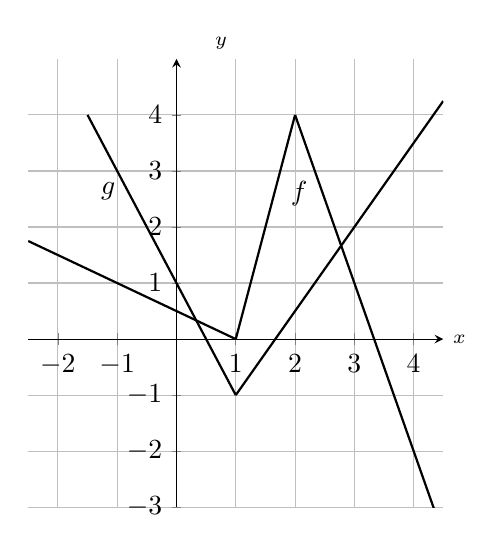
\begin{tikzpicture}
\begin{axis}[axis y line=middle,axis x line=middle, ymajorgrids=true, xmajorgrids=true, ymin=-3,ymax=5, xmin=-2.5,xmax=4.5, name=myplot, xscale=1/1.3, ytick={-3,-2,-1,0,1,2,3,4}]
\addplot [draw={\colorone}, domain=-1.5:1,thick] {-2*x+1}; 
\addplot [draw={\colorone}, domain=1:4.5,thick] {1.5*x-2.5};
\addplot [draw={\colortwo}, domain=-2.5:1, thick] {-.5*x+.5};
\node[label={30:{$g$}}] at (axis cs:-1.6,2.2) {};
\addplot [draw={\colortwo}, domain=1:2, thick] {4*x-4};
\node[label={30:{$f$}}] at (axis cs:1.6,2.1) {};
\addplot [draw={\colortwo}, domain=2:4.5, thick] {-3*x+10};
\end{axis}
\node [right] at (myplot.right of origin) {\scriptsize $x$};
\node [above] at (myplot.above origin) {\scriptsize $y$};
\end{tikzpicture}\\*
\begin{tabular}{ll}
(a) $(f \circ g)'(-1)$ & (b) $(g \circ f)'(0)$ \\
(c) $(g \circ g)'(-1)$ & (d) $(f \circ f)'(4)$
\end{tabular}
}{(a) $6$  \qquad (b) $1$ \qquad (c) $-4$ \qquad (d) $1.5$
}

\exercise{\[
\begin{array}{cccccc}
x && f(x) & \fp(x) & g(x) & g'(x) \\\midrule
1&&4&5&4&5\\
4&&0&7&1&\frac12\\
6&&6&4&6&3
\end{array}
\]
Use the given table of values for $f$, $g$, $\fp$, and $g'$ to find
\begin{enumerate}
\item $(f \circ g)'(6)$
\item $(g \circ f)'(1)$
\item $(g \circ g)'(6)$
\item $(f \circ f)'(1)$
\end{enumerate}}{(a) $12$  \quad (b) $2.5$ \quad (c) $9$ \quad (d) $35$
}

\exerciseset{In Exercises}{, find the equations of tangent and normal lines to  the graph of the function at the given point. Note: the functions here are the same as in Exercises \ref{exer:02_05_06} through \ref{exer:02_05_09}.
}{

\exercise{$f(x) = (4x^3-x)^{10}$ at $x=0$
}{Tangent line: $y=0$

Normal line: $x=0$
}

\exercise{$f(t) = (3t-2)^5$ at $t=1$
}{Tangent line: $y=15(t-1)+1$

Normal line: $y=-1/15(t-1)+1$
}

\exercise{$g(\theta) = (\sin\theta+\cos\theta)^3$ at $\theta = \pi/2$
}{Tangent line: $y=-3(\theta - \pi/2)+1$

Normal line: $y=1/3(\theta - \pi/2)+1$
}

\exercise{$h(t) = e^{3t^2+t-1}$ at $t=-1$
}{Tangent line: $y=-5e(t+1)+e$

Normal line: $y=1/(5e)(t+1)+e$
}

}
\exercise{Compute $\ds \frac{d}{dx}\big(\ln (kx)\big) $ two ways: 
\begin{enumerate}
\item		Using the Chain Rule, and 
\item		by first using the logarithm rule $\ln (ab) = \ln a + \ln b$, then taking the derivative.
\end{enumerate}
}{In both cases the derivative is the same: $1/x$. 
}

\exercise{Compute $\ds \frac{d}{dx}\big(\ln (x^k)\big) $ two ways: 
\begin{enumerate}
\item		Using the Chain Rule, and 
\item		by first using the logarithm rule $\ln (a^p) = p\ln a$, then taking the derivative.
\end{enumerate}
}{In both cases the derivative is the same: $k/x$. 
}

\exercise{Use the Chain Rule to prove the following:
\begin{enumerate}
\item The derivative of an even function is an odd function.
\item The derivative of an odd function is an even function.
\end{enumerate}
}{Let $g(x)=-x$.  Then
\begin{enumerate}
\item $f\circ g=f$, so $\fp(-x)=\fp\circ g(x)=-\fp\circ g(x)g'(x)=-(f\circ g)'(x)=-\fp(x)$
\item $f\circ g=-f$, so $\fp(-x)=\fp\circ g(x)=-\fp\circ g(x)g'(x)=-(f\circ g)'(x)=\fp(x)$
\end{enumerate}
}

\exercise{Use the Chain Rule and Product Rule to give an alternative proof of the Quotient Rule. (Hint: write $f(x)/g(x)$ as $f(x) \cdot [g(x)]^{-1})$.
}{Let $h(x)=x^{-1}$.  Then
$\dfrac{d}{dx}\dfrac{f(x)}{g(x)}=\dfrac{d}{dx}\left[f(x)\cdot h(g(x))\right]=\dfrac{d}{dx}\left[f(x)\right]\cdot h(g(x))+f(x)\cdot\dfrac{d}{dx}\left[h(g(x))\right]=\fp(x)\cdot h(g(x))+f(x)\cdot h'(g(x))\cdot g'(x)=\fp(x)[g(x)]^{-1}-f(x)[g(x)]^{-2}g'(x)=\dfrac{\fp(x)g(x)-f(x)g'(x)}{[g(x)]^2}$
}

\exercise{Use the Chain Rule to express the second derivative of $f(g(x))$ in terms of first and second derivatives of $f$ and $g$.
}{$[f(g(x))]''
=[\fp(g(x))g'(x)]'
=[\fp(g(x))]'g'(x)+\fp(g(x))g''(x)
=\fpp(g(x))g'(x)g'(x)+\fp(g(x))g''(x)
=\fpp(g(x))[g'(x)]^2+\fp(g(x))g''(x)$
}

\printreview

\exercise{The ``wind chill factor'' is a measurement of how cold it ``feels'' during cold, windy weather. Let $W(w)$ be the wind chill factor, in degrees Fahrenheit, when it is $25^\circ$F outside with a wind of $w$ mph. 
	\begin{enumerate}
	\item		What are the units of $W\primeskip'(w)$?
	\item		What would you expect the sign of $W\primeskip'(10)$ to be?
	\end{enumerate}
}{\begin{enumerate}
\item		$^\circ$ F/mph
\item		The sign would be negative; when the wind is blowing at 10 mph, any increase in wind speed will make it feel colder, i.e., a lower number on the Fahrenheit scale.
\end{enumerate}
}

\exercise{Find the derivatives of %the following functions.
%\begin{enumerate}
%\item
$f(x) = x^2e^x\cot x$
%\item	$g(x) = 2^x3^x4^x$
%\end{enumerate}
}{%\begin{enumerate}
%\item
$2xe^x\cot x + x^2e^x\cot x - x^2e^x\csc^2 x$
%\item		$\ln(48)48^x$
%\end{enumerate}
}
